\documentclass[12pt, conference]{IEEEtran}
\IEEEoverridecommandlockouts
% The preceding line is only needed to identify funding in the first footnote. If that is unneeded, please comment it out.
\usepackage{cite}
\usepackage{amsmath,amssymb,amsfonts}
\usepackage{algorithmic}
\usepackage{graphicx}
\usepackage{textcomp}
\usepackage{verbatim}
\usepackage{xcolor}
\usepackage{setspace}
\usepackage{url}
\usepackage{subcaption}
\usepackage{hyperref}

\def\BibTeX{{\rm B\kern-.05em{\sc i\kern-.025em b}\kern-.08em
    T\kern-.1667em\lower.7ex\hbox{E}\kern-.125emX}}

\begin{document}

\title{A Combined ViT-FNN Model for Bird Species Classification from Audio Recordings}

\author{\IEEEauthorblockN{Bardia Parmoun}
\IEEEauthorblockA{\textit{Systems and Computer Engineering} \\
\textit{Carleton University}\\
Ottawa, Canada \\
bardiaparmoun@cmail.carleton.ca}
\and
\IEEEauthorblockN{Huda Sheikh}
\IEEEauthorblockA{\textit{Systems and Computer Engineering} \\
\textit{Carleton University}\\
Ottawa, Canada \\
hudasheikh@cmail.carleton.ca}
\and
\IEEEauthorblockN{Nadia Ahmed}
\IEEEauthorblockA{\textit{Systems and Computer Engineering} \\
\textit{Carleton University}\\
Ottawa, Canada \\
nadianahmed@cmail.carleton.ca}
\and
\IEEEauthorblockN{Prianna Rahman}
\IEEEauthorblockA{\textit{Systems and Computer Engineering} \\
\textit{Carleton University}\\
Ottawa, Canada\\
priannarahman@cmail.carleton.ca}
}

\maketitle

\doublespacing

\section{Introduction}
This document is a detailed summary of the final project implementation for the BIOM/SYSC 5405 course, Pattern Classification and Experiment Design. The goal of this project was to recognize the chirps of 10 different bird species from 1-minute recordings. The following birds were considered: 
\begin{itemize}
\item AMRO - American Robin
\item BHCO - Brown-headed Cowbird
\item CHSW - Chimney Swift
\item EUST - European Starling
\item GRCA - Gray Catbird
\item HOSP - House Sparrow
\item HOWR - House Wren
\item NOCA - Northern Cardinal
\item RBGU - Ring-billed Gull
\item RWBL - Red-winged Blackbird
\end{itemize}

The data included recordings from 11 different locations and were gathered in such a way that each recording included zero to multiple different bird species. The team had access to data from three different years, 2021 to 2023 (each year having around 3000 recordings). For this project, the data from the years 2021 and 2022 were used for training, and the data from 2023 were held back as blind test data to measure the model's performance.

\section{Methodology}
\subsection{Approach}

For the final project, the team was assigned to identify the specific birds heard in multiple audio recordings, given data from various locations and years. This was a multi-label problem, as each recording could have multiple bird sounds. In addition, both the audio recordings and CSV files with the corresponding spectrograms were given, making the problem multi-modal as well. Ultimately, the team decided to use meta-learning and ensemble learning techniques to combine predictions from both a Feed-forward Neural Network (FNN) and Vision Transformer (ViT). Here is a quick overview of the approach that was used:

\begin{figure}[htbp]
\centerline{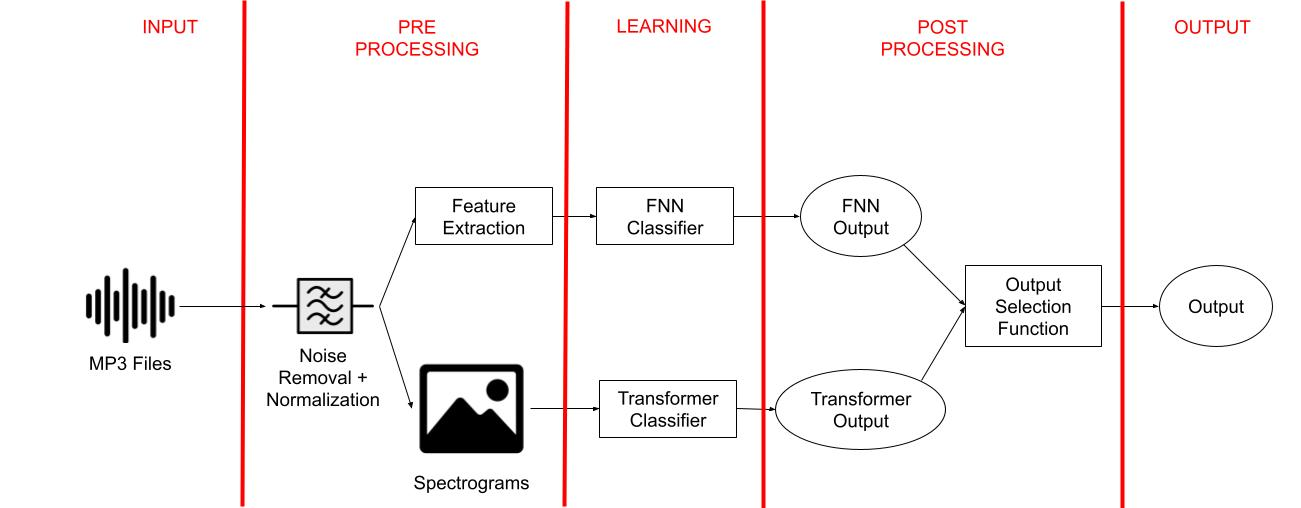
\includegraphics[width=\columnwidth]{figures/approach_diagram.jpg}}
\caption{A diagram of the team's approach.}
\label{appraoch}
\end{figure}

First, the given MP3 files were processed by applying noise reduction and normalization. Then, proper audio features such as mel-frequency cepstral coefficients (MFCCs), chroma, spectral contrast, and location were extracted for the FNN model. In addition, the processed audio was turned into a spectrogram for the ViT model. The outputs of each model were then combined through hard voting to come up with the final prediction. Each aspect of this method will be discussed further in the following sections.

\subsection{Data Pre-Processing}
At the beginning of the project, two sources of data were given: MP3 and the corresponding CSV files containing spectrogram data of the recordings. When listening to the audio recordings, it was noticed that bird sounds were largely drowned out by the noise (traffic noise, other environmental noise, etc.). To hopefully reduce the effects of the noise, the audio was pre-processed by performing band-pass filtering. Bird sounds are known to range from roughly 1000 Hz to 8000 Hz \cite{allaboutbirds}. Traffic noise is usually in the range of 500 to 2500 Hz \cite{trafficnoise}. To be slightly aggressive, all audio recordings were band-passed from 3000 Hz to 8000 Hz. To perform this noise reduction, a Butterworth band-pass filter with an order of 3 in \texttt{MATLAB} was used. After processing the audio, the bird sounds were much more noticeable, and the noise was significantly reduced. The team then proposed to amplify the bird sounds further by applying a gain to each of the audio recordings. Although this did work in intensifying the bird sounds, it did cause some undesirable effects such as increased processing time and clipping. Ultimately, it was decided that reducing the noise was sufficient enough. To avoid the effects of clipping from filtering the audio, the recordings were normalized so the amplitude did not exceed the range [-1 1]. Since pre-processing was performed on the audio, the spectrograms were created directly from the recordings, rather than from the provided CSV files. An example of the effects of this pre-processing can be seen in Figure \ref{fig:spectrograms}. In Fig. 2 (a), there is a noticeable amount of irrelevant data (blue areas of the spectrogram), and the bird sounds are mainly located at lower frequencies (red areas of the spectrogram). Fig. 2 (b) shows a cleaned version of the spectrogram, after bandpass filtering and data normalization. In this spectrogram, the bird chirp pattern is much more clear (shown in red).

\begin{figure}[htbp]
    \centering
    \begin{subfigure}[b]{0.3\textwidth}
        \centering
        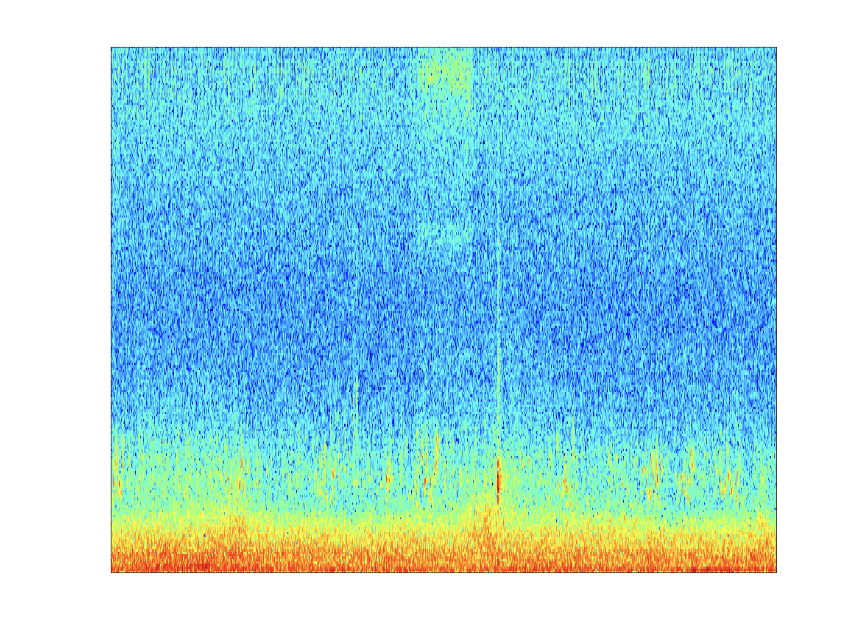
\includegraphics[width=\linewidth]{figures/spectrogram_original.png}
        \caption{Original Spectrogram}
        \label{fig:OriginalSpectrogram}
    \end{subfigure}
    \hfill
    \begin{subfigure}[b]{0.24\textwidth}
        \centering
        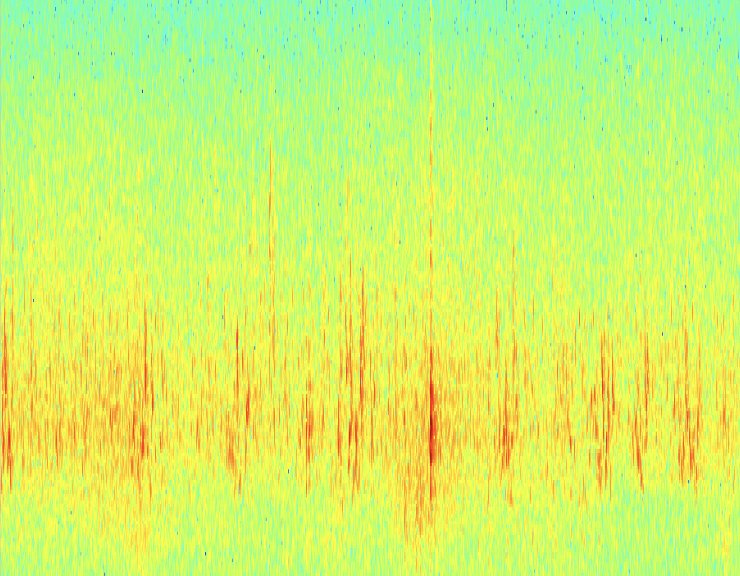
\includegraphics[width=\linewidth]{figures/spectrogram_clean.png}
        \caption{Cleaned Spectrogram}
        \label{fig:CleanedSpectrogram}
    \end{subfigure}
    \caption{(a) The original spectrogram and (b) The original spectrogram filtered through a band-pass filter.}
    \label{fig:spectrograms}
\end{figure}

As mentioned previously, the team's proposed method was to combine both an FNN model and ViT model. The audio recordings were fed to the FNN model, and the spectrograms were fed to the ViT model. Using both sources of data ultimately led to more accurate predictions.

For feature extraction, the most relevant features from the audio were extracted for classification using the \texttt{librosa} library. As noted earlier, these include the MFCCs, chroma, and spectral contrast. MFCCs show the power spectrum of a signal by taking the audio and applying a series of Fourier transforms and transformations to find the proper coefficients. These help define frequency patterns and harmonics. Chroma is another useful feature. For this feature, the audio spectrum is split into 12 distinct bins, which represent the 12 distinct semitones across all octaves \cite{chromafeatures}. The chroma can help differentiate between different pitches. The spectral contrast is the difference between peak and valley energies within sub-bands of an audio signal \cite{librosa}. A high spectral contrast indicates a sound closer to a pure tone, and a low spectral contrast is closer to noise. In addition, the location of each recording was added as an additional feature to the feature set by encoding each location into a number from 1 to 11. This ensured that the model was aware of the bird species that were not present in certain locations.

\subsection{Feature Importance}

The chart in Figure \ref{fig:feature_importance} illustrates Feature Importance Based on Mutual Information, which measures how much each feature contributes to predicting bird species. Higher mutual information scores indicate stronger relevance to the classification task.

\begin{figure}[h!]
    \centering
    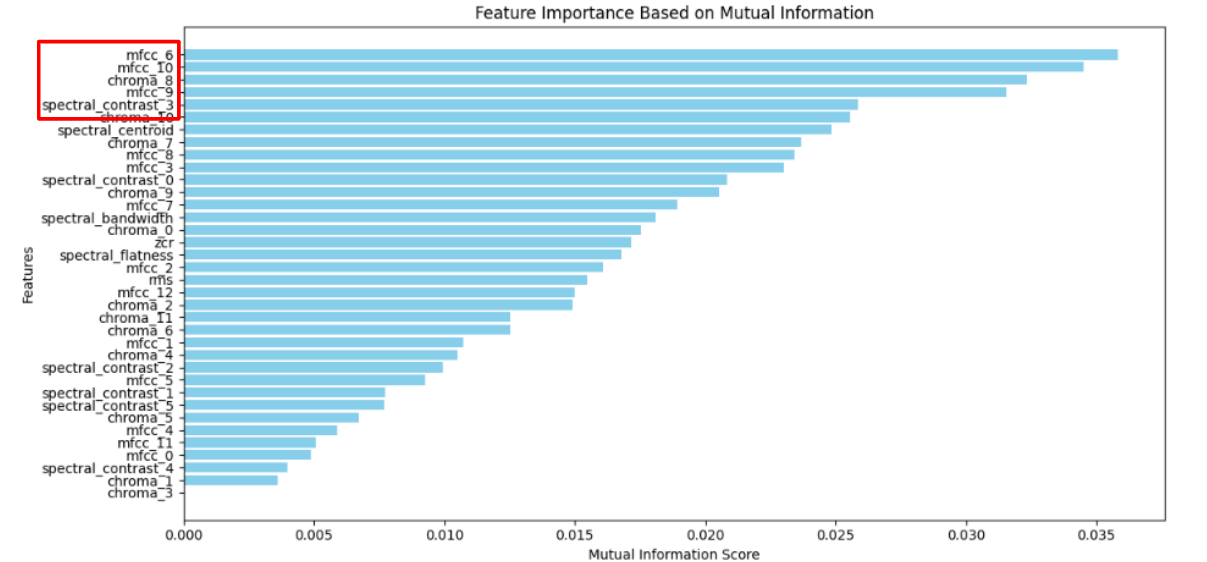
\includegraphics[width=\linewidth]{figures/feature_importance.png}
    \caption{Feature Importance Based on Mutual Information. Higher scores indicate stronger relevance of features for predicting bird species.}
    \label{fig:feature_importance}
\end{figure}

The top three features identified are:
\begin{itemize}
    \item \textbf{MFCC\_6}: Captures spectral properties, highlighting tonal and frequency details.
    \item \textbf{MFCC\_10}: Reinforces the importance of spectral features in vocal classification.
    \item \textbf{Chroma\_8}: Represents pitch class distribution, capturing tonal and harmonic structures.
\end{itemize}

These features can be categorized into two main types:
\begin{itemize}
    \item \textbf{MFCCs}: Focus on frequency and spectral details to analyze tonal qualities. MFCCs, particularly MFCC\_6 and MFCC\_10, emphasize the fine-grained spectral properties that are essential for identifying unique vocal patterns in bird calls.
    \item \textbf{Chroma Features}: Highlight pitch patterns and melodic structures. Chroma\_8, in particular, emphasizes harmonic and tonal content, making it useful for identifying repetitive tonal patterns in bird vocalizations.
\end{itemize}

Together, MFCCs and chroma features complement each other. MFCCs provide a detailed spectral analysis, while chroma features emphasize tonal and harmonic patterns. This combination is crucial for distinguishing bird vocalizations, as spectral properties help separate tonal bird calls from environmental noise, and harmonic structures enhance the detection of melodic patterns unique to bird species.


\subsection{Meta-Learning}
Meta-learning is a machine-learning approach that helps models perform well on new tasks by learning from patterns across different datasets or models \cite{meta}. It focuses on combining strengths from multiple models to improve overall accuracy and adaptability, especially when data is limited \cite{meta}. In this project, meta-learning was used by combining the predictions of two models: an FNN trained on audio features and a ViT trained on spectrograms. These models focused on different types of data, and their predictions were combined using a hard voting method, which averaged their outputs to make final decisions. To ensure balanced and consistent predictions, the team optimized the decision threshold. This approach allowed the combined model to take advantage of each individual model's strengths, resulting in better overall performance and reliability in identifying bird species from audio recordings and spectrograms. 

\subsection{Implementation}
To implement this project, the group utilized \texttt{Python} and \texttt{Google Colab}. Additionally, the team used popular \texttt{Python} libraries such as \texttt{PyTorch} and \texttt{TensorFlow} to implement the ViT and FNN models. Furthermore, as previously mentioned, the team implemented various \texttt{MATLAB} scripts for the pre-processing phase. A \texttt{GitHub} repository containing the complete implementation of the project is located at:

\url{https://github.com/bardia-p/Bird-Classifier}

\section{Experimentation}
\subsection{Training and Validation}
In the beginning stages of the project, the team decided to work with ViT and long short-term memory (LSTM) models. However, after some experimentation with sequential and non-sequential data, the team moved to using FNN instead of LSTM because of its better performance. This is due to the fact that each audio recording has one label, and not a label for each timestamp within the recording.  

As previously mentioned, raw audio recordings were pre-processed to extract numerical feature vectors. For the FNN, these extracted features were combined with a location-specific feature (representing the geographical context) to form the final input vector. For the ViT, spectrograms were generated from the audio data, divided into fixed-size patches, and embedded into a 768-dimensional space for input. The training data consisted of labeled audio recordings from multiple locations. Each audio file was processed to generate the appropriate input format for the respective model. Each of the models was trained for a fixed number of epochs, with early stopping mechanisms based on validation performance to avoid overfitting. The team chose to perform training using stochastic gradient descent (\texttt{SGD}) with momentum of $0.9$, rather than adaptive moment estimation (\texttt{ADAM}).

A separate validation set was created, ensuring no overlap with the training data. Validation performance was monitored using metrics like accuracy, precision, recall, and F1-score. Validation loss trends were used to adjust hyperparameters, including learning rates, dropout rates, and regularization strength.

The team also optimized and refined the hyperparameters using iterative experiments. The learning rate, dropout rate, \texttt{L2} regularization strength, and transformer-specific settings (e.g., patch size, embedding dimension) were tuned based on validation performance. \texttt{ReduceLROnPlateau} was also used to dynamically adjust the learning rate during training, ensuring the models could fine-tune effectively.

Figure \ref{fig:metrics} shows the final metrics collected during training. Further steps can be taken to improve these metrics, such as regularization for the ViT.

\begin{figure}[htbp]
\centerline{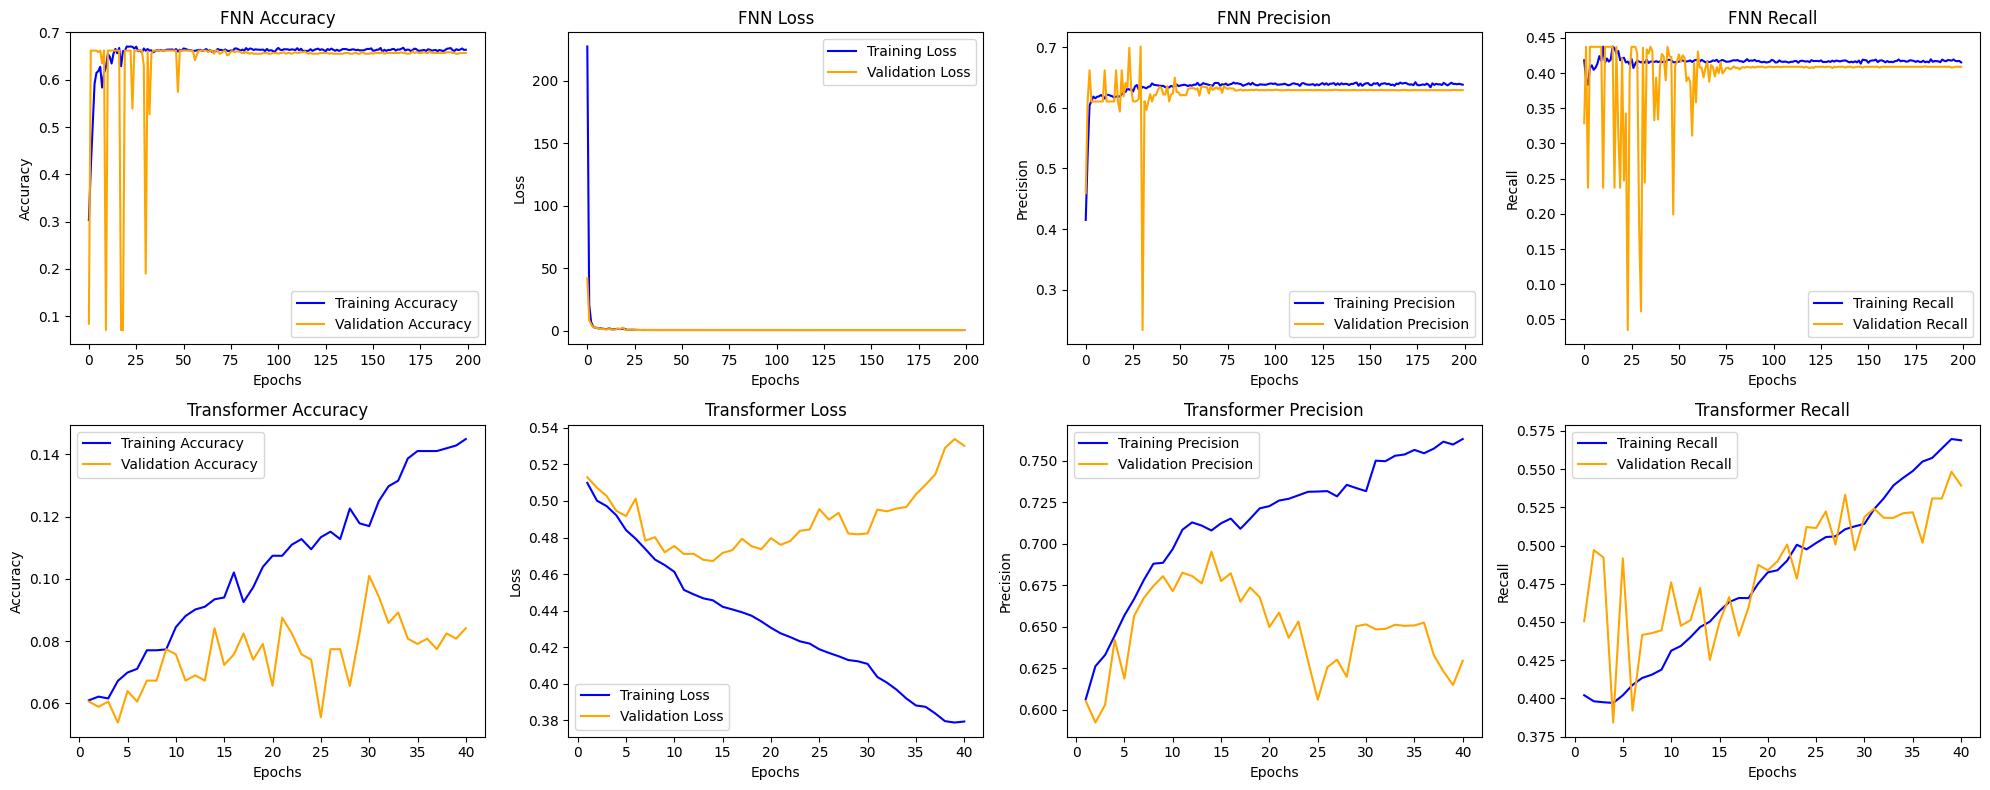
\includegraphics[width=\columnwidth]{figures/metrics_all_data.png}}
\caption{A summary of the metrics of the transformer and the FNN during training.}
\label{fig:metrics}
\end{figure}

\subsection{Estimation of Model Performance}
After predictions from both models were averaged to create combined probabilities, various thresholds (ranging from 0 to 1) were tested to convert these probabilities into binary predictions, and the F1-score was calculated for each threshold. The F1-score (micro average) is a performance metric that calculates the harmonic mean of precision and recall across all classes, treating every sample equally regardless of its class labels. It uses the true positives, false positives, and false negatives across all classes and then computes the precision and recall to calculate the F1-score.

This metric is useful for addressing class imbalance because it ensures that each sample contributes equally to the overall score, regardless of the class distribution. Unlike the macro average, which gives equal weight to each class, the micro average prevents smaller classes from being dominated by larger classes. Therefore, the micro-averaged F1-score provides a balanced assessment of how well the model handles both majority and minority classes in imbalanced datasets.

The best threshold for maximizing the F1-score was recorded for that fold. After all folds, the mean and standard deviation of the F1-scores was calculated in order to reflect the model's average performance and variability across different splits. This cross-validation approach ensured a thorough evaluation of the model’s performance. Additionally, the mean and standard deviation of the selected thresholds were computed to assess consistency. The final selected threshold was $0.148 \pm 0.01$. While the final threshold value reflects data imbalance, its low variability indicates consistent threshold selection across folds.

In the end, the estimate of the meta-model's performance based on the five-fold cross validation process was $59.2 \pm 0.1$. 

\section{Testing}
\subsection{Testing Process}
As previously mentioned, the team used data provided from 2023 to verify the model. The team utilized the models that were trained during the experimentation phase (200 epochs for the FNN and 40 epochs for the ViT conducted on $80\%$ of the data collected in 2021 and 2022). To prepare the test data, the same pre-processing scripts were run on it. After that, the cleaned audio files and spectrograms were fed through the same feature extraction process. It is worth mentioning that the team made sure to apply the same encoding logic, that was done during the training process, to the location labels. 

After running both models on the test data, the team combined their results by applying the same meta-learning technique of hard voting. Finally, to obtain the final binary predictions, the mean value of the best threshold that was obtained during cross-validation (0.15) to the final weights was applied. 

\subsection{Results}
After submitting the test results, the team received an F1-score of $59.16$ which was very similar to the estimate that was submitted ($59.2 \pm 0.1$). This resulted in a very high precision of $39.862$ for the team. These results indicate that the model's performance was as expected and quite consistent when faced with new data.

\section{Discussion and Reflections}
\subsection{Strengths}
As mentioned in the testing section, a big strength of the developed model is consistency and satisfactory performance when faced with blind test data. The team believes that various factors contributed to this:

First, the team utilized a lot of data to train the models. Through the precise feature selection process, both 2021 and 2022 datasets were utilized which greatly reduced the meta-model's risk of overfitting. In addition, it should be noted that the team avoided using too many features since those would also increase the risk of overfitting.

Additionally, as mentioned in the experimentation section, the team tried different threshold values to account for the inconsistent behaviours of the models. In other words, each model was trained separately with a threshold of 0.5 to ensure they learned as much as possible about the data; however, after combining the two, the team decided to reduce the overall threshold to around 0.15 since it was found that the model was underfitting.  

Furthermore, the team decided to utilize meta-learning which allowed for the usage of both audio files and the spectrograms. Training two separate models and combining them also reduced the variance of the overall model, since the FNN and ViT behaved quite differently and were given very different inputs. The overall bias of the model is also very low, as both the FNN and ViT are deep learning models that do not make a lot of assumptions about the shape of the distribution. An observation that the team had which can clearly be seen in Figure \ref{fig:metrics} is that the FNN model was particularly good at precision (shown by its validation precision) and similarly the ViT model was good at recall (shown by its validation recall metric). This meant by averaging the two models together the team was able to get consistent and satisfactory precision and recall values which together resulted in a consistent F1-score. 

To reduce the risk of overfitting even further, the team performed five-fold cross-validation on the data. In each fold, both classifiers were given the same train, validation, and test data to obtain the best F1 score and threshold that can be calculated by both models. The team repeatedly adjusted the various hyper-parameters until these values were sufficiently consistent.

Finally, the team made the conscious decision to tackle the class imbalance problem through providing the additional location feature as opposed to utilizing popular methods such as class weights or under-sampling. This is due to the fact that some bird species might not be available in certain locations meaning using a class weights or under-sampling on all the data will incorrectly punish the model for learning useful information about the non-minority classes. The team also noticed that the distribution of data changed greatly between 2021 and 2022, meaning there is a good chance that the data from 2023 did not have a similar distribution to them. This is another reason why the use of class weights might lead to overfitting. On the other hand, the use of location as a feature ensures that the model only learns about the overpopulated classes when applicable and would be another factor to distinguish the minority classes from each other.

\subsection{Challenges}
The team noticed that the training accuracies of both the FNN and the ViT were always around $70\%$ no matter the number of epochs or the hyperparameters used. This indicates a lack of data and shows that there is still room for the model to grow given more data or better features. This is especially true since there are $2^{10} = 1024$ possible label combinations for the data, but the team was only provided with around 3000 samples per year which included a lot of similar label combinations. If the data had more examples and more unique labels, the mvariation would help the model tp fprm better pattern associations. In the future, the team would like to experiment using more features or using external feature extraction libraries such as the \texttt{Wavelet} library \cite{wavelet}.

The team faced difficulties with the quality of the data. Unfortunately, the original recordings included a lot of noise. In addition, the recordings seemed to include other background sounds in them. Some of these challenges were mitigated with cleanup scripts; however, there is still room to improve the quality of these audio files.

Additionally, the data could have been formatted better. Audio recordings are ideal for LSTMs and other models that support sequential data; however, the data only had one label per recording indicating that there is a bird chirp somewhere in the recording. This means that the data is essentially no longer sequential, since we need to consider the recording as a whole. It would have been beneficial if specific timestamps were given for each recording indicating where the different bird chirps occur. This would make the data much better for models such as the LSTM.

Finally, the team was provided with limited time and resources to train these models. This factor became especially prevalent when it came to training the ViT. Transformers usually need a lot of training time, even on T4 GPUs. As such, the team did not have sufficient time or resources to be able to properly tune this model and regularize its output. If given another opportunity, the team would like to experiment with a simpler model such as a convolutonal neural network (CNN) to train the spectrogram data.

\subsection{Conclusions}
In conclusion, the team believes that the approach discussed in this report can serve as a starting point for training a model to solve this problem. In this project, it has been shown that it is possible to develop a meta-learning model that behaves consistently when faced with new data. In addition, the team's approach showed how the use of meta-learning and proper data pre-processing can improve the performance of a model. Finally, it was shown that using both spectrograms and audio files will be greatly beneficial in improving and stabilizing the performance of machine learning models. This suggests that the next iterations of the project should continue looking into methods that can utilize both input formats. An example of that could be using an LSTM or RNN model on the audio files and using a CNN on the spectrograms and combining the results.

\section{Contributions}

\subsection{Report Contributions}

Table \ref{table:report} outlines the contributions made toward the preparation and writing of this report:

\begin{table}[h!]
\centering
\caption{Report Contributions}
\resizebox{\columnwidth}{!}{%
\begin{tabular}{|p{4cm}|p{5cm}|}
\hline
\textbf{Section} & \textbf{Contributors} \\ \hline
Introduction & Bardia \\ \hline
Methodology & Prianna, Huda \\ \hline
Experimentation & Nadia, Huda, Prianna \\ \hline
Testing & Bardia \\ \hline
Discussion and Reflections & Bardia, Nadia \\ \hline
Contributions & Nadia \\ \hline
Figures and Visualizations & Bardia, Huda, Nadia, Prianna \\ \hline
References and Citation Management & Bardia, Huda, Nadia, Prianna \\ \hline
Proofreading and Editing & Bardia, Huda, Nadia, Prianna  \\ \hline
\end{tabular}
\label{table:report}
}
\end{table}

\subsection{Project Contributions}

Table \ref{table:project} outlines the contributions made to the execution of the project:

\begin{table}[h!]
\centering
\caption{Project Contributions}
\resizebox{\columnwidth}{!}{%
\begin{tabular}{|p{4cm}|p{5cm}|}
\hline
\textbf{Task} & \textbf{Contributors} \\ \hline
Data Preparation and Preprocessing & Prianna, Huda, Nadia \\ \hline
Feature Exploration & Nadia, Huda \\ \hline
Feature Extraction & Huda, Prianna \\ \hline
FNN Training and Validation & Bardia, Huda \\ \hline
ViT Training and Validation & Nadia, Huda, Bardia \\ \hline
Blind Test Evaluation & Bardia \\ \hline
\end{tabular}
\label{table:project}
}
\end{table}


\section*{Acknowledgment}

This project was completed to fulfill the project requirements for BIOM/SYSC 5405, Pattern Classification and Experiment Design. This project could not have been complete without support from Professor James Green, and the dataset provided by Chris Dennison and Dr. Rachel Buxton from the Department of Biology at Carleton University. 

\bibliography{references.bib}
\bibliographystyle{ieeetr}
\vspace{12pt}

\end{document}
